\documentclass[tikz,border=3mm]{standalone}
\usepackage{fontspec}
\usepackage{amsmath}
\usepackage{xcolor}
\usepackage{tikz}
\usetikzlibrary{
  arrows.meta,
  backgrounds,
  calc,
  decorations.pathreplacing,
  fit,
  positioning,
  shapes.geometric,
  shapes.symbols
}

\IfFontExistsTF{Comic Sans MS}
  {\setmainfont{Comic Sans MS}}
  {\setmainfont{TeX Gyre Heros}}

\tikzset{
  >={Stealth[length=2.2mm,width=1.6mm]},
  figure title/.style={font=\fontsize{14}{16}\selectfont,align=center},
  figure subtitle/.style={font=\fontsize{8}{10}\selectfont,align=center},
  figure label/.style={font=\fontsize{7.5}{9}\selectfont,align=center},
  figure tiny/.style={font=\fontsize{6.2}{7.4}\selectfont,align=center},
  data flow/.style={-Stealth,line width=1.0pt},
  control flow/.style={-Stealth,dashed,line width=.8pt},
  projection/.style={densely dotted,line width=.8pt},
  compute/.style={rectangle,rounded corners=1.6mm,line width=.8pt,
    minimum height=.72cm,inner xsep=5pt,inner ysep=3pt,figure label},
  event/.style={diamond,aspect=1.3,line width=.8pt,inner sep=1.4pt,figure tiny},
  store/.style={cylinder,shape border rotate=90,aspect=.28,line width=.8pt,
    minimum height=.78cm,figure label},
  state/.style={circle,line width=.8pt,minimum size=.72cm,figure tiny},
  fusion/.style={regular polygon,regular polygon sides=6,line width=.8pt,
    minimum width=1.4cm,figure tiny}
}

\definecolor{ink}{HTML}{16324D}
\definecolor{navy}{HTML}{183B60}
\definecolor{teal}{HTML}{087F87}
\definecolor{violet}{HTML}{8060AB}
\definecolor{amber}{HTML}{BC8320}
\definecolor{coral}{HTML}{C46786}
\definecolor{graphite}{HTML}{64778B}
\definecolor{divider}{HTML}{D5E0E9}
\definecolor{paper}{HTML}{FFFFFF}
\definecolor{navybg}{HTML}{F0F5FA}
\definecolor{tealbg}{HTML}{EBF7F4}
\definecolor{violetbg}{HTML}{F3EFF8}
\definecolor{amberbg}{HTML}{FFF6E5}
\definecolor{pale}{HTML}{F8FBFC}

\tikzset{
  concord backbone/.style={draw=navy,fill=navybg,line width=.9pt},
  concord conditioning/.style={draw=teal,fill=tealbg,line width=.9pt},
  concord context/.style={draw=violet,fill=violetbg,line width=.9pt},
  concord supervision/.style={draw=amber,fill=amberbg,line width=.9pt},
  concord projection/.style={trapezium,trapezium left angle=70,trapezium right angle=110,
    concord context,minimum width=2.8cm,minimum height=.62cm,text width=2.35cm,
    inner sep=1.5pt,font=\fontsize{6.6}{7.8}\selectfont,align=center},
  concord fusion/.style={regular polygon,regular polygon sides=6,concord conditioning,
    minimum size=.75cm,text width=1.15cm,inner sep=.6pt,
    font=\fontsize{6.3}{7.4}\selectfont,align=center},
  concord store/.style={cylinder,shape border rotate=90,aspect=.28,concord supervision,
    minimum width=3.0cm,minimum height=.7cm,text width=2.4cm,inner sep=1.5pt,
    font=\fontsize{6.6}{7.8}\selectfont,align=center},
  concord detached/.style={-Stealth,dashed,line width=.85pt,draw=amber},
  concord data/.style={-Stealth,line width=1.0pt},
  concord shared/.style={densely dotted,line width=.8pt,draw=graphite}
}


\begin{document}
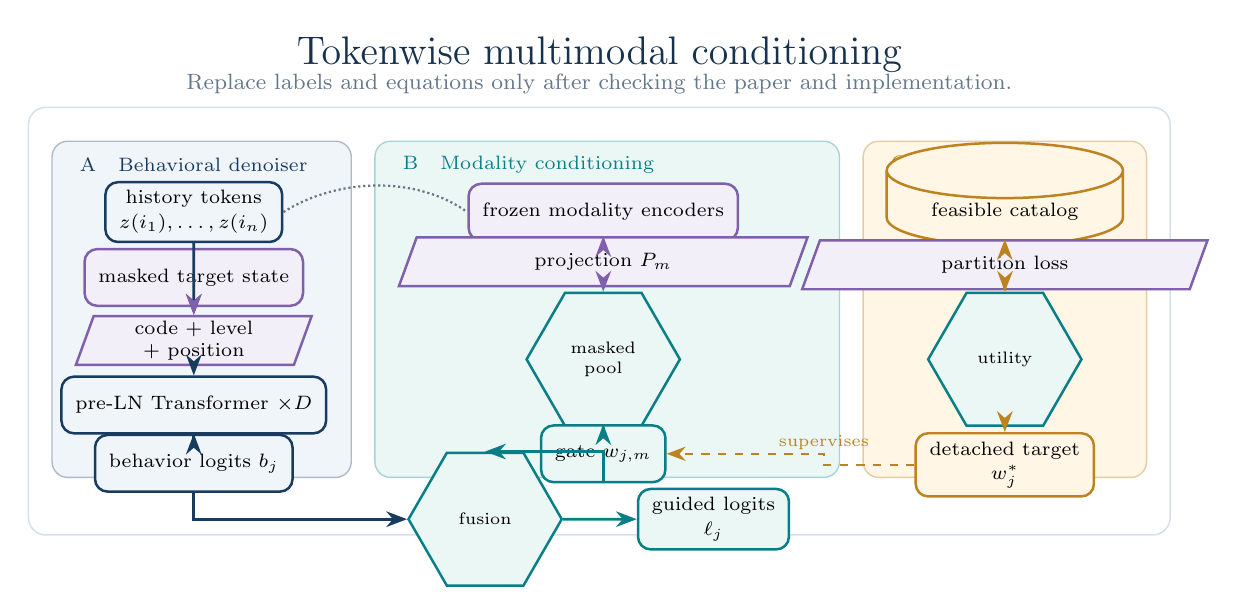
\begin{tikzpicture}[x=1cm,y=1cm]
  % CONCORD-Rec grammar: color = computational role; shape = object type.
  \node[figure title,text=ink] at (7.5,6.45) {Tokenwise multimodal conditioning};
  \node[figure subtitle,text=graphite] at (7.5,6.08)
    {Replace labels and equations only after checking the paper and implementation.};

  \begin{scope}[on background layer]
    \fill[rounded corners=2.2mm,fill=paper,draw=divider,line width=.55pt]
      (.25,.35) rectangle (14.75,5.78);
    \fill[rounded corners=2mm,fill=navybg,draw=navy!35,line width=.5pt]
      (.55,1.08) rectangle (4.35,5.35);
    \fill[rounded corners=2mm,fill=tealbg,draw=teal!35,line width=.5pt]
      (4.65,1.08) rectangle (10.55,5.35);
    \fill[rounded corners=2mm,fill=amberbg,draw=amber!40,line width=.5pt]
      (10.85,1.08) rectangle (14.45,5.35);
  \end{scope}

  \node[figure label,text=navy,anchor=west] at (.78,5.05) {A\quad Behavioral denoiser};
  \node[figure label,text=teal,anchor=west] at (4.88,5.05) {B\quad Modality conditioning};
  \node[figure label,text=amber,anchor=west,font=\fontsize{7}{8}\selectfont] at (11.08,5.05) {C\quad Offline utility};

  \node[compute,concord backbone] (history) at (2.35,4.45)
    {history tokens\\$z(i_1),\ldots,z(i_n)$};
  \node[compute,concord context] (target) at (2.35,3.62)
    {masked target state};
  \node[concord projection] (embed) at (2.35,2.82)
    {code + level + position};
  \node[compute,concord backbone] (denoiser) at (2.35,2.00)
    {pre-LN Transformer $\times D$};
  \node[compute,concord backbone] (logits) at (2.35,1.26)
    {behavior logits $b_j$};
  \draw[concord data,draw=navy] (history) -- (embed);
  \draw[concord data,draw=violet] (target) -- (embed);
  \draw[concord data,draw=navy] (embed) -- (denoiser);
  \draw[concord data,draw=navy] (denoiser) -- (logits);

  \node[compute,concord context] (encoders) at (7.55,4.45)
    {frozen modality encoders};
  \node[concord projection] (projection) at (7.55,3.82)
    {projection $P_m$};
  \node[concord fusion] (pool) at (7.55,2.58)
    {masked pool};
  \node[compute,concord conditioning] (gate) at (7.55,1.38)
    {gate $w_{j,m}$};
  \draw[concord data,draw=violet] (encoders) -- (projection);
  \draw[concord data,draw=violet] (projection) -- (pool);
  \draw[concord data,draw=teal] (pool) -- (gate);

  \node[concord store] (support) at (12.65,4.45)
    {feasible catalog};
  \node[concord projection] (loss) at (12.65,3.78)
    {partition loss};
  \node[concord fusion] (utility) at (12.65,2.58)
    {utility};
  \node[compute,concord supervision] (targetw) at (12.65,1.24)
    {detached target\\$w_j^*$};
  \draw[concord data,draw=amber] (support) -- (loss);
  \draw[concord data,draw=amber] (loss) -- (utility);
  \draw[concord data,draw=amber] (utility) -- (targetw);
  \draw[concord detached] (targetw.west) -- ++(-1.15,0) |- (gate.east)
    node[pos=.2,above,figure tiny,text=amber]{supervises};

  \node[concord fusion] (fuse) at (6.05,.55) {fusion};
  \node[compute,concord conditioning] (guided) at (8.95,.55) {guided logits\\$\ell_j$};
  \draw[concord data,draw=navy] (logits.south) |- (fuse.west);
  \draw[concord data,draw=teal] (gate.south) |- (fuse.north);
  \draw[concord data,draw=teal] (fuse) -- (guided);
  \draw[concord shared] (history.east) .. controls (4.2,4.9) and (5.2,4.9) .. (encoders.west);

\end{tikzpicture}
\end{document}
